% ============================================================
% 12-de-casteljau-makie-explained.tex
% Compile with:  pdflatex -shell-escape 12-de-casteljau-makie-explained.tex
% The PNG must be in the same folder. Run twice for TOC.
% ============================================================

\documentclass[12pt, a4paper]{article}

\usepackage[T1]{fontenc}
\usepackage[utf8]{inputenc}
\usepackage{lmodern}
\usepackage[top=2.5cm, bottom=2.5cm, left=2.8cm, right=2.8cm]{geometry}
\usepackage{graphicx}
\usepackage{float}
\usepackage[dvipsnames]{xcolor}

\definecolor{codebg}{RGB}{248,248,248}
\definecolor{rulecolor}{RGB}{180,180,180}
\definecolor{examplebg}{RGB}{240,248,255}
\definecolor{examplerule}{RGB}{100,149,237}
\definecolor{notebg}{RGB}{255,250,230}
\definecolor{noterule}{RGB}{210,180,50}
\definecolor{diffbg}{RGB}{240,255,240}
\definecolor{diffrule}{RGB}{80,160,80}
\definecolor{samebg}{RGB}{245,245,245}
\definecolor{samerule}{RGB}{160,160,160}

\usepackage{minted}
\setminted[julia]{
  bgcolor=codebg, frame=leftline, framerule=1.5pt,
  rulecolor=rulecolor, linenos=false, fontsize=\small,
  breaklines=true, tabsize=4, style=friendly,
}

\usepackage{amsmath}
\usepackage{amssymb}
\usepackage{tikz}
\usetikzlibrary{shapes.geometric, arrows.meta, positioning}
\usepackage{mdframed}

\newmdenv[backgroundcolor=examplebg, linecolor=examplerule,
  linewidth=1.5pt, leftline=true, rightline=false,
  topline=false, bottomline=false,
  innerleftmargin=10pt, innerrightmargin=8pt,
  innertopmargin=6pt, innerbottommargin=6pt,
  skipabove=6pt, skipbelow=4pt]{examplebox}

\newmdenv[backgroundcolor=notebg, linecolor=noterule,
  linewidth=1.5pt, leftline=true, rightline=false,
  topline=false, bottomline=false,
  innerleftmargin=10pt, innerrightmargin=8pt,
  innertopmargin=6pt, innerbottommargin=6pt,
  skipabove=6pt, skipbelow=4pt]{notebox}

\newmdenv[backgroundcolor=diffbg, linecolor=diffrule,
  linewidth=1.5pt, leftline=true, rightline=false,
  topline=false, bottomline=false,
  innerleftmargin=10pt, innerrightmargin=8pt,
  innertopmargin=6pt, innerbottommargin=6pt,
  skipabove=6pt, skipbelow=4pt]{diffbox}

\newmdenv[backgroundcolor=samebg, linecolor=samerule,
  linewidth=1.5pt, leftline=true, rightline=false,
  topline=false, bottomline=false,
  innerleftmargin=10pt, innerrightmargin=8pt,
  innertopmargin=6pt, innerbottommargin=6pt,
  skipabove=6pt, skipbelow=4pt]{samebox}

\usepackage[colorlinks=true, linkcolor=black, urlcolor=MidnightBlue]{hyperref}
\usepackage{booktabs}
\usepackage{needspace}
\usepackage{parskip}
\usepackage{titlesec}
\usepackage{fancyhdr}
\usepackage{datetime2}

\titleformat{\section}
  {\large\bfseries\color{MidnightBlue}}{\thesection.}{0.6em}{}
  [\vspace{-4pt}\rule{\linewidth}{0.4pt}]
\titleformat{\subsection}
  {\normalsize\bfseries\color{BrickRed}}{\thesubsection.}{0.5em}{}
\titleformat{\subsubsection}
  {\normalsize\bfseries}{\thesubsubsection.}{0.5em}{}

\pagestyle{fancy}
\fancyhf{}
\rhead{\textcolor{gray}{\small 12-de-casteljau-makie-explained}}
\lhead{\textcolor{gray}{\small De Casteljau --- CairoMakie}}
\cfoot{\thepage}
\renewcommand{\headrulewidth}{0.3pt}

\newcommand{\cd}[1]{\texttt{#1}}

\title{%
  \vspace{1cm}
  {\LARGE\bfseries De Casteljau Algorithm}\\[0.4em]
  {\large Quadratic B\'ezier --- CairoMakie Visualisation}\\[0.4em]
  {\large Code and Plot Explanation for Julia Beginners}\\[0.4em]
  {\normalsize\texttt{12-de-casteljau-makie.jl}}
}
\author{E.R.\ Nurwijayadi}
\date{\DTMtoday}

\begin{document}

\maketitle
\thispagestyle{empty}

\begin{center}
\textit{Directed and curated by E.R.\ Nurwijayadi.
Code and explanations AI-generated.}
\end{center}

\begin{center}
\begin{minipage}{0.85\textwidth}
\small
This document explains \cd{12-de-casteljau-makie.jl},
the CairoMakie counterpart to \cd{12-de-casteljau-plots.jl}.
The De Casteljau algorithm, all data structures, and all
computed values are identical to the Plots.jl version.
This document is fully self-contained but focuses on the
API differences from Plots.jl.
The math section is kept brief --- refer to
\cd{12-de-casteljau-plots-explained} for the full
geometric explanation and all data tables.
\end{minipage}
\end{center}

\vspace{1em}\hrule\vspace{1.5em}
\tableofcontents
\newpage


% =============================================================
\needspace{8\baselineskip}
\section{The Plot}
% =============================================================

\begin{figure}[H]
  \centering
  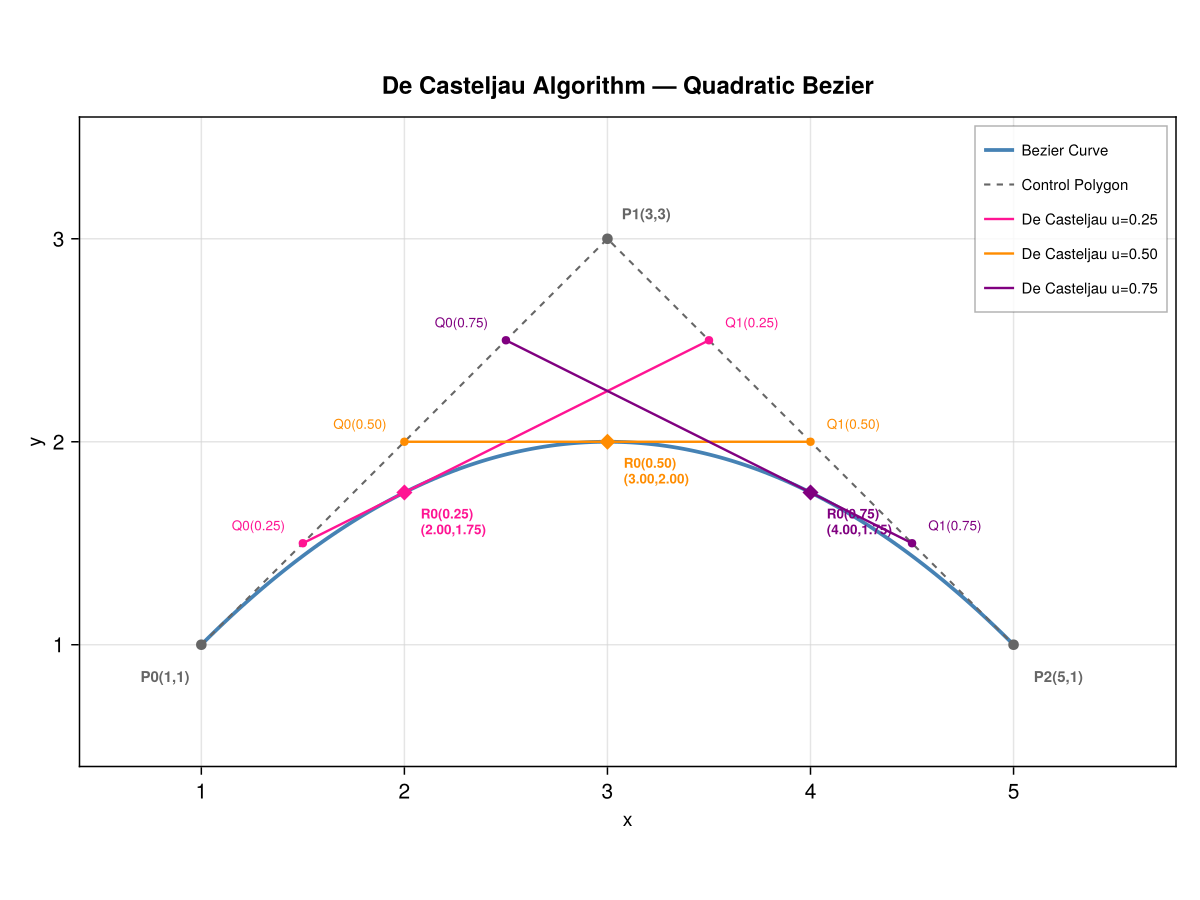
\includegraphics[width=0.95\linewidth]{12-bezier_decasteljau-makie.png}
  \caption{De Casteljau algorithm at $u=0.25$ (pink),
           $u=0.50$ (orange), $u=0.75$ (purple).
           Rendered with CairoMakie.}
  \label{fig:decasteljau-makie}
\end{figure}


% =============================================================
\needspace{8\baselineskip}
\section{Visual Differences from the Plots.jl Version}
% =============================================================

\begin{center}
\begin{tabular}{lll}
\toprule
Element & Plots.jl & CairoMakie \\
\midrule
Frame & Four-sided box & Open axes \\
Title font & Normal weight & \textbf{Bold}, \cd{titlesize=16} \\
Title spacing & No gap control & \cd{titlegap=12} adds breathing room \\
Control polygon & Gray30 & Gray40 (slightly lighter) \\
Control markers & Size 6 & Size 10 (more prominent) \\
$Q$ dots & Size 5 & Size 8 \\
$R_0$ diamond & Size 7 & Size 12 (clearly visible) \\
Resolution & 800$\times$600 px & 1200$\times$900 px (\cd{px\_per\_unit=1.5}) \\
Legend & \cd{legend=:topright} in \cd{plot()} & \cd{axislegend(ax)} \\
\bottomrule
\end{tabular}
\end{center}

The Makie version has consistently larger markers and a
bolder title, giving the construction points more visual
weight against the higher-resolution canvas.


% =============================================================
\needspace{8\baselineskip}
\section{What Is Identical to the Plots.jl Version}
% =============================================================

\begin{samebox}
\begin{tabular}{lp{9.5cm}}
\toprule
Component & Note \\
\midrule
\cd{CONTROL\_POINTS}, \cd{U\_SNAPSHOTS}, \cd{SNAPSHOT\_COLORS} &
  Byte-for-byte identical. \\
\cd{DeCasteljauQuadratic} struct \& constructor &
  Identical. \\
\cd{lerp} &
  Identical one-liner broadcast function. \\
\cd{steps} &
  Identical --- same three \cd{lerp} calls, same named tuple return. \\
\cd{dc\_curve} &
  Identical --- same \cd{.level2} field access pattern. \\
Colour constants &
  \cd{COLOR\_CURVE = :steelblue}; \cd{COLOR\_POLYGON = :gray40}
  (vs \cd{:gray30} in Plots.jl). \\
\cd{CTRL\_NAMES}, \cd{CTRL\_OFFSET}, \cd{Q\_OFFSETS} &
  Identical. \\
All data tables &
  \cd{l0}, \cd{l1}, \cd{r0} values are the same.
  See \cd{12-de-casteljau-plots-explained} for full tables. \\
\bottomrule
\end{tabular}
\end{samebox}


% =============================================================
\needspace{8\baselineskip}
\section{The Math (Brief Summary)}
% =============================================================

The De Casteljau algorithm evaluates a B\'ezier curve at
parameter $u$ by two rounds of linear interpolation.

\textbf{Level 1:}
$Q_0 = (1-u)P_0 + uP_1$, \quad $Q_1 = (1-u)P_1 + uP_2$

\textbf{Level 2:}
$R_0 = (1-u)Q_0 + uQ_1$ \quad (the curve point)

The \cd{lerp} function computes one linear interpolation.
\cd{steps(dc, u)} calls \cd{lerp} three times and returns
the three levels as a named tuple.
See \cd{12-de-casteljau-plots-explained} for the full
geometric explanation and worked examples at all three
$u$ values.


% =============================================================
\needspace{8\baselineskip}
\section{\texttt{draw\_and\_save} --- The Makie Drawing API}
% =============================================================

\needspace{5\baselineskip}
\subsection{Figure and Axis: \texttt{titlegap}}

\begin{minted}{julia}
fig = Figure(size = (800, 600), backgroundcolor = :white)

ax = Axis(fig[1, 1],
    title          = "De Casteljau Algorithm - Quadratic Bezier",
    titlesize      = 16,
    titlegap       = 12,
    xlabel         = "x",
    ylabel         = "y",
    xlabelsize     = 13,
    ylabelsize     = 13,
    limits         = (0.4, 5.8, 0.4, 3.6),
    aspect         = DataAspect(),
    xgridcolor     = (:lightgray, 0.6),
    ygridcolor     = (:lightgray, 0.6),
    backgroundcolor = :white,
)
\end{minted}

Most attributes here were explained in
\cd{11-bezier-quadratic-makie-explained}.
The one new attribute is \cd{titlegap}.

\textbf{\cd{titlegap = 12}:}
Controls the vertical gap (in points) between the title
text and the top edge of the plot area.
Without this, Makie places the title very close to the
axis frame, which can look cramped when the title is
large (\cd{titlesize = 16}).
A value of 12 adds comfortable breathing room.

\begin{diffbox}
\textbf{Plots.jl} has no direct equivalent to \cd{titlegap}.
The title spacing is handled automatically by the layout engine
and cannot be fine-tuned per-plot.

\textbf{CairoMakie} exposes \cd{titlegap} as an explicit
\cd{Axis} attribute, giving you pixel-level control.
\end{diffbox}

\needspace{5\baselineskip}
\subsection{Curve and Control Polygon}

\begin{minted}{julia}
# Bezier curve
cpts = dc_curve(dc)
lines!(ax, cpts[:,1], cpts[:,2],
    color = COLOR_CURVE, linewidth = 2.5, label = "Bezier Curve")

# Control polygon
l0 = steps(dc, 0.0).level0
lines!(ax, l0[:,1], l0[:,2],
    color = COLOR_POLYGON, linestyle = :dash,
    linewidth = 1.4, label = "Control Polygon")
scatter!(ax, l0[:,1], l0[:,2],
    color = COLOR_POLYGON, markersize = 10, strokewidth = 0)
\end{minted}

Identical in logic to the Plots.jl version.
Makie requires two separate calls (\cd{lines!} and
\cd{scatter!}) for the control polygon line and its
markers, as established in script~11.

The control polygon markers are \cd{markersize = 10}
here (vs 6 in Plots.jl), producing the larger grey
dots visible at $P_0$, $P_1$, $P_2$ in the Makie plot.

\needspace{5\baselineskip}
\subsection{Control Point Labels}

\begin{minted}{julia}
for (i, (name, (dx, dy))) in enumerate(zip(CTRL_NAMES, CTRL_OFFSET))
    text!(ax, l0[i,1]+dx, l0[i,2]+dy,
        text     = name,
        color    = COLOR_POLYGON,
        fontsize = 10,
        font     = :bold,
    )
end
\end{minted}

The loop pattern --- \cd{enumerate(zip(names, offsets))} ---
is identical to the Plots.jl version.

One small difference: the label colour here is
\cd{COLOR\_POLYGON} (\cd{:gray40}), giving
labels the same grey as the control polygon.
In the Plots.jl version, \cd{COLOR\_CTRL = :crimson}
made the labels red like the polygon markers.
In this Makie version the control polygon is grey,
so the labels match that grey.

\needspace{5\baselineskip}
\subsection{The Snapshot Loop}

\begin{minted}{julia}
for (u, color) in zip(u_snapshots, colors)
    s  = steps(dc, u)
    l1 = s.level1
    r0 = s.level2

    # Level-1 segment
    lines!(ax, l1[:,1], l1[:,2],
        color = color, linewidth = 1.6,
        label = @sprintf("De Casteljau u=%.2f", u))

    # Level-1 Q dots
    scatter!(ax, l1[:,1], l1[:,2],
        color = color, markersize = 8, strokewidth = 0)

    # Level-2 R0 diamond
    scatter!(ax, [r0[1]], [r0[2]],
        color = color, marker = :diamond,
        markersize = 12, strokewidth = 0)

    # Q0, Q1 labels
    for (j, (qname, (dx, dy))) in enumerate(zip(["Q0","Q1"], Q_OFFSETS))
        text!(ax, l1[j,1]+dx, l1[j,2]+dy,
            text = @sprintf("%s(%.2f)", qname, u),
            color = color, fontsize = 9)
    end

    # R0 label
    text!(ax, r0[1]+0.08, r0[2]-0.22,
        text  = @sprintf("R0(%.2f)\n(%.2f,%.2f)", u, r0[1], r0[2]),
        color = color, fontsize = 9, font = :bold)
end
\end{minted}

The loop structure and logic are identical to the Plots.jl
version.
The API differences follow the established Makie pattern:

\begin{center}
\begin{tabular}{lll}
\toprule
Operation & Plots.jl & CairoMakie \\
\midrule
Draw line segment & \cd{plot!(plt, ...)} & \cd{lines!(ax, ...)} \\
Draw scatter dots & \cd{scatter!(plt, ...)} & \cd{scatter!(ax, ...)} \\
Suppress legend entry & \cd{label = false} & \textit{(no label keyword passed)} \\
Place text & \cd{annotate!(plt, x, y, text(...))} & \cd{text!(ax, x, y, text=...)} \\
\bottomrule
\end{tabular}
\end{center}

\begin{notebox}
\textbf{Suppressing legend entries in Makie.}
In Plots.jl, \cd{label = false} explicitly hides a layer
from the legend.
In Makie, simply omitting the \cd{label} keyword from a
\cd{scatter!} or \cd{lines!} call is sufficient ---
unlabelled elements never appear in the legend.
This is why the $Q$ dots and $R_0$ diamonds in this
script have no \cd{label} argument at all.
\end{notebox}

\begin{examplebox}
\textbf{The \cd{[r0[1]]} single-point scatter idiom (same as Plots.jl):}

\cd{r0 = s.level2} is a length-2 vector, e.g.\ \cd{[2.0, 1.75]}.

\cd{scatter!(ax, [r0[1]], [r0[2]], ...)} wraps each coordinate
in a length-1 vector to satisfy Makie's requirement that
$x$ and $y$ arguments are arrays, not scalars.

Same pattern as the Plots.jl version --- both libraries
require arrays for scatter coordinates.
\end{examplebox}

\needspace{5\baselineskip}
\subsection{Legend and Save}

\begin{minted}{julia}
axislegend(ax,
    position        = :rt,
    labelsize       = 10,
    framecolor      = (:black, 0.3),
    backgroundcolor = (:white, 0.8),
)

save(filename, fig, px_per_unit = 1.5)
println("Saved: $filename")
display(fig)
println("Press Enter to close...")
readline()
\end{minted}

Identical to \cd{11-bezier-quadratic-makie-explained}.
\cd{axislegend} reads the five labelled elements
(Bezier Curve, Control Polygon, and three De Casteljau
snapshots) and builds the legend automatically.
The unlabelled \cd{scatter!} calls for dots and diamonds
are correctly excluded.


% =============================================================
\needspace{8\baselineskip}
\section{Entry Point}
% =============================================================

\begin{minted}{julia}
function main()
    dc = DeCasteljauQuadratic(CONTROL_POINTS)
    draw_and_save(dc, U_SNAPSHOTS, SNAPSHOT_COLORS,
                  "12-bezier_decasteljau-makie.png")
end

main()
\end{minted}

Identical structure to the Plots.jl version.

\begin{notebox}
\textbf{How to run:}
\begin{minted}{julia}
julia 12-de-casteljau-makie.jl
\end{minted}
Saves \cd{12-bezier\_decasteljau-makie.png} and opens a window.
Press Enter to close.
\end{notebox}


% =============================================================
\needspace{8\baselineskip}
\section{Complete API Reference: This Script vs Plots.jl}
% =============================================================

\begin{center}
\begin{tabular}{p{3.5cm}p{4.8cm}p{4.8cm}}
\toprule
Operation & \cd{12-de-casteljau-plots.jl} & \cd{12-de-casteljau-makie.jl} \\
\midrule
Create canvas &
  \cd{plt = plot(...)} &
  \cd{fig = Figure(...)} \\[4pt]
Create axes &
  (combined with canvas) &
  \cd{ax = Axis(fig[1,1], ...)} \\[4pt]
Title gap &
  (not available) &
  \cd{titlegap = 12} \\[4pt]
Draw line &
  \cd{plot!(plt, xs, ys)} &
  \cd{lines!(ax, xs, ys)} \\[4pt]
Draw markers &
  \cd{scatter!(plt, xs, ys)} &
  \cd{scatter!(ax, xs, ys)} \\[4pt]
Suppress legend &
  \cd{label = false} &
  (omit \cd{label} keyword) \\[4pt]
Text annotation &
  \cd{annotate!(plt, x, y, text(...))} &
  \cd{text!(ax, x, y, text=...)} \\[4pt]
Single point &
  \cd{scatter!(plt, [x], [y])} &
  \cd{scatter!(ax, [x], [y])} \\[4pt]
Legend &
  \cd{legend=:topright} in \cd{plot()} &
  \cd{axislegend(ax, position=:rt)} \\[4pt]
Save &
  \cd{savefig(plt, filename)} &
  \cd{save(filename, fig, px\_per\_unit=1.5)} \\
\bottomrule
\end{tabular}
\end{center}

\vspace{2em}\hrule\vspace{0.5em}
{\small\textcolor{gray}{%
Explanation for \texttt{12-de-casteljau-makie.jl}
\textbar{} Directed and curated by E.R.\ Nurwijayadi
\textbar{} Code and explanations AI-generated}}

\end{document}
